\documentclass{article}
\usepackage[T1]{fontenc}
\usepackage[utf8]{inputenc}
\usepackage[submission]{ismir} % Remove the "submission" option for camera-ready version
\usepackage{amsmath,amssymb,cite,url}
\usepackage{graphicx}
\usepackage{color}
\usepackage{tikz}
\usetikzlibrary{arrows.meta,positioning,shapes.geometric}

\title{Score-Based Hierarchical Phrase-Boundary Prediction with Performance-Derived Supervision}

\oneauthor
  {Anonymous Authors}
  {Anonymous Affiliations\\anonymous@ismir.net}
\def\authorname{F. Author, S. Author, and T. Author}

\sloppy % please retain sloppy command for improved formatting

\begin{document}

\maketitle

\begin{abstract}
Hierarchical phrase structure is important for expressive-timing analysis and generation, yet phrase boundaries are rarely explicit in the score. This paper presents a score-only model for hierarchical phrase-boundary prediction trained from performance-derived supervision. Using MazurkaBL, aligned beat-level timing curves are converted into nested performer-level boundary layers by recursive group analysis and reorganized into five weighted top-down cumulative targets. Beat-synchronous MusicXML features are aggregated to the beat grid, and a 1D convolutional neural network performs beat-level sequence tagging from score context alone under a strict outer-piece protocol, achieving mean union precision $0.87$, weighted recall $0.41$, and consensus recall $0.51$ on three held-out Mazurkas. A controlled blind evaluation by three musicians of varying training shows that lenient acceptance of model boundaries reaches $0.87$--$0.93$ across raters while no random control marker is judged as required, and a post hoc tempo-curve reconstruction analysis shows that the predicted boundaries still capture broad expressive-timing shape. These results support score-based hierarchical phrase-boundary prediction as an interpretable structural module for downstream expressive-performance generation and as a useful aid for piano learning and performance preparation.
\end{abstract}

\section{Introduction}\label{sec:introduction}

Hierarchical phrase structure is central to how performers shape expressive timing and how analysts read musical form~\cite{Todd1985ExpressiveTiming,Li2016ExpressiveTimingThesis}. Phrase boundaries are simultaneously an analytical output, a control handle for expressive-timing generation, and a practical aid for piano learners and performers preparing a work. Yet they are rarely written explicitly in the score, and direct annotation is subjective, labor-intensive, and of low inter-annotator agreement at finer levels~\cite{McFee2017HierarchicalAnnotations,Wang2017CrowdsourcingSegmentation}. Large-scale supervised phrase-boundary prediction from the score therefore cannot straightforwardly inherit the conventional labeled-corpus paradigm.

Existing score-based segmentation methods fall into three lines. Rule-based models rooted in GTTM~\cite{LerdahlJackendoff1983} operationalize local notational cues, with Cambouropoulos's LBDM~\cite{Cambouropoulos2001LBDM} targeting local change points and Temperley's Grouper~\cite{Temperley2001Cognition} producing phrase-level groupings. Statistical models such as IDyOM~\cite{Pearce2010Melodic} reframe boundary detection as locating points of high predictive uncertainty. Neural sequence taggers combine CNN or TCN encoders with CRF decoders~\cite{Guan2018Melodic,Zhang2021SymbolicMelody,Jiang2022HierarchicalMetrical}. Two gaps remain for the grouping (phrase) case: supervision depends on subjective human annotation, and hierarchy is treated as discrete decoder states rather than a target property.

These gaps are addressed by a score-only hierarchical phrase-boundary predictor trained from performance-derived supervision. Aligned Mazurka performances from MazurkaBL~\cite{Kosta18MazurkaBL} are used only as structural evidence: beat-level tempo curves are converted, via recursive window-based analysis~\cite{Li2016ExpressiveTimingThesis}, into five nested performer-averaged boundary layers and reorganized into a weighted top-down cumulative target. A 1D convolutional neural network is trained on beat-synchronous MusicXML features under a strict outer-piece protocol, requiring no performance signal at test time. The trained detectors are additionally applied qualitatively to a Mozart piano-sonata movement to inspect out-of-domain behavior.

The paper makes three contributions. The first is a procedure for deriving multi-level phrase-boundary supervision from aligned performance timing, sidestepping the low agreement of direct hierarchical annotation. The second is a weighted top-down cumulative target that encodes hierarchical consistency in label space, enabling a 1D-CNN to produce five coarse-to-fine detectors nested by design under a strict outer-piece protocol. Finally, we report a controlled human evaluation by music-school instructors and a post hoc tempo-curve reconstruction analysis showing that the predicted hierarchy retains enough structural information to support downstream expressive-timing generation and to serve as a readable aid for piano learning and performance preparation.

\section{Data and Boundary Annotation}\label{sec:data}

\subsection{Mazurka Corpus}\label{subsec:mazurka_corpus}

The experiments use MazurkaBL~\cite{Kosta18MazurkaBL}, a corpus of Chopin Mazurka performances with aligned beat-level expressive information. It contains score-aligned loudness, beat, and expressive-marking information for approximately 2,000 Chopin Mazurka recordings. According to the dataset construction procedure, beat locations are first annotated in a reference recording for each piece and then transferred to the remaining recordings through audio-to-audio alignment using chroma and chroma-onset features \cite{Ewert2009ChromaOnsetSync}. In the present study, the symbolic score serves as model input and the aligned performance realizations are used only to derive phrase-boundary supervision. Following the curated piece split used in the experiments, the working subset contains 44 Mazurka pieces and 1999 aligned performance realizations, and all 44 score files are in the \(3/4\) time signature. The basic unit of analysis is the score beat, so that symbolic features, performance-derived boundary annotations, and model predictions are all defined on the same beat grid.

\subsection{Hierarchical Boundary Annotation from Performance MIDI}\label{subsec:boundary_annotation}

The hierarchical boundary labels are derived from aligned performance MIDI through the multi-level tempo-boundary analysis of Li~\cite{Li2016ExpressiveTimingThesis}, summarized in Figure~\ref{fig:boundary_pipeline}. These signals are treated as performance-derived hierarchical boundary targets rather than as literal ground-truth phrase boundaries.

\begin{figure}[t]
  \centering
  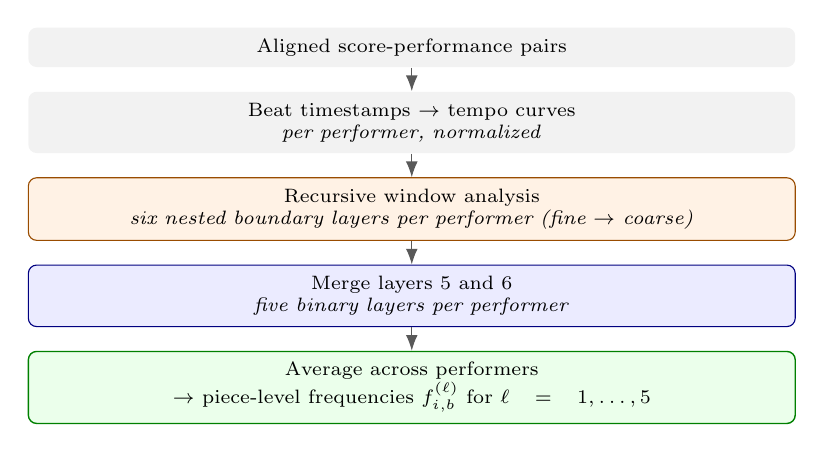
\begin{tikzpicture}[
    every node/.style={font=\scriptsize},
    input/.style={
      fill=gray!10,
      rounded corners=3pt, align=center,
      text width=0.78\linewidth, inner sep=4pt
    },
    extract/.style={
      draw=orange!60!black, line width=0.4pt,
      fill=orange!10,
      rounded corners=3pt, align=center,
      text width=0.78\linewidth, inner sep=4pt
    },
    aggregate/.style={
      draw=blue!50!black, line width=0.4pt,
      fill=blue!8,
      rounded corners=3pt, align=center,
      text width=0.78\linewidth, inner sep=4pt
    },
    output/.style={
      draw=green!50!black, line width=0.5pt,
      fill=green!8,
      rounded corners=3pt, align=center,
      text width=0.78\linewidth, inner sep=4pt
    },
    arrow/.style={-{Latex[length=2mm]}, line width=0.45pt, gray!70!black}
  ]

    \node[input] (input) {Aligned score-performance pairs};
    \node[input, below=0.30cm of input] (timing)
      {Beat timestamps $\to$ tempo curves\\\textit{per performer, normalized}};
    \node[extract, below=0.30cm of timing] (extract)
      {Recursive window analysis\\\textit{six nested boundary layers per performer (fine $\to$ coarse)}};
    \node[aggregate, below=0.30cm of extract] (aggregate)
      {Merge layers 5 and 6\\\textit{five binary layers per performer}};
    \node[output, below=0.30cm of aggregate] (target)
      {Average across performers\\$\to$ piece-level frequencies $f_{i,b}^{(\ell)}$ for $\ell=1,\dots,5$};

    \draw[arrow] (input)     -- (timing);
    \draw[arrow] (timing)    -- (extract);
    \draw[arrow] (extract)   -- (aggregate);
    \draw[arrow] (aggregate) -- (target);

  \end{tikzpicture}
  \caption{Boundary-annotation pipeline. Aligned tempo curves are processed by a recursive window analysis to extract six nested per-performer layers, merged to five layers, and averaged across performers to give piece-level frequencies $f_{i,b}^{(\ell)}$.}
  \label{fig:boundary_pipeline}
\end{figure}

For each performer, aligned beat timestamps are converted into inter-beat durations and then into a beat-level tempo curve. Implausible values are removed, missing values are linearly interpolated, and the curve is smoothed with a centered three-beat moving-average window. The pipeline is instantiated with grouping schedule $[3,2,2,2,2,2]$, which reflects the metrical regularity of the Mazurka corpus: all 44 score files are in $3/4$, so the first aggregation step spans one bar, after which increasingly broader layers are formed by pairwise grouping. Let $s=(s_1,\ldots,s_6)=(3,2,2,2,2,2)$ denote these grouping factors. The cumulative block width at level $\ell$ is $w_\ell = \prod_{r=1}^\ell s_r$, yielding $(3,6,12,24,48,96)$ beats; level $\ell$ partitions the beat axis into consecutive blocks $\mathcal{B}_k^{(\ell)}$ of width $w_\ell$.

Level 1 boundaries are obtained by detecting valleys directly on the beat-level tempo curve. At each higher level $\ell \geq 2$, the salience of the $k$-th block is computed on the $w_\ell$ mean-normalized raw tempo values inside the block, following the RMS-minus-standard-deviation formulation of Li:
\begin{equation}
g_{k}^{(\ell)} =
\sqrt{\frac{1}{w_{\ell}}\sum_{j=1}^{w_{\ell}} \left(\tilde{\tau}_{k,j}^{(\ell)}\right)^2}
- \mathrm{std}\!\left(\tilde{\tau}_{k,1:w_{\ell}}^{(\ell)}\right),
\end{equation}
where $\tilde{\tau}_{k,j}^{(\ell)}$ is the mean-normalized tempo at the $j$-th raw beat inside the $k$-th level-$\ell$ block. The RMS term selects blocks whose tempo sits close to the performer-specific mean (a global-minimum candidate at this scale), while subtracting the standard deviation rewards blocks whose internal tempo varies, preventing large windows from masking shorter local minima.

Li's per-layer probability outputs are adapted into nested per-layer binary masks: valleys of $g_k^{(\ell)}$ are traced back to single beats by recursively selecting the minimum-salience child, and nesting is enforced by cumulative union from the coarsest layer downward. The original sixth layer is very sparse and largely overlaps the fifth, so the two are merged into a single coarsest layer, yielding five performer-level boundary layers $L_1,\ldots,L_5$. 

\subsection{Learning Targets and Evaluation Protocol}\label{subsec:targets_protocol}

The learning problem is defined as beat-level prediction from score features. $\mathbf{x}_{i,b}$ denotes the symbolic feature vector at beat $b$ of piece $i$ and $y_{i,p,b}^{(\ell)} \in \{0,1\}$ indicates whether performer $p$ places a level-$\ell$ boundary at the same beat. Rather than imitating any single performer, the model learns a performer-aggregated boundary tendency, summarized for each level by
\begin{equation}
f_{i,b}^{(\ell)} = \frac{1}{P_i}\sum_{p=1}^{P_i} y_{i,p,b}^{(\ell)},
\end{equation}
the fraction of performers who place a level-$\ell$ boundary at beat $b$ in piece $i$. These beat-level frequencies are the starting point for the cumulative detector targets defined in Section~\ref{subsec:cumulative_targets}.

A fixed piece-level split is used, with M06-1, M06-2, and M06-3 reserved for clean outer evaluation and the remaining 41 Mazurkas used for development; the exact training and model-selection procedure is described in Section~\ref{subsec:protocol}.

\section{Methods}\label{sec:methods}

This section describes the score-based feature representation, the weighted top-down cumulative target construction, the convolutional predictor, and the training and inference procedure. Figure~\ref{fig:method_pipeline} summarizes the learning pipeline.

\begin{figure}[t]
  \centering
  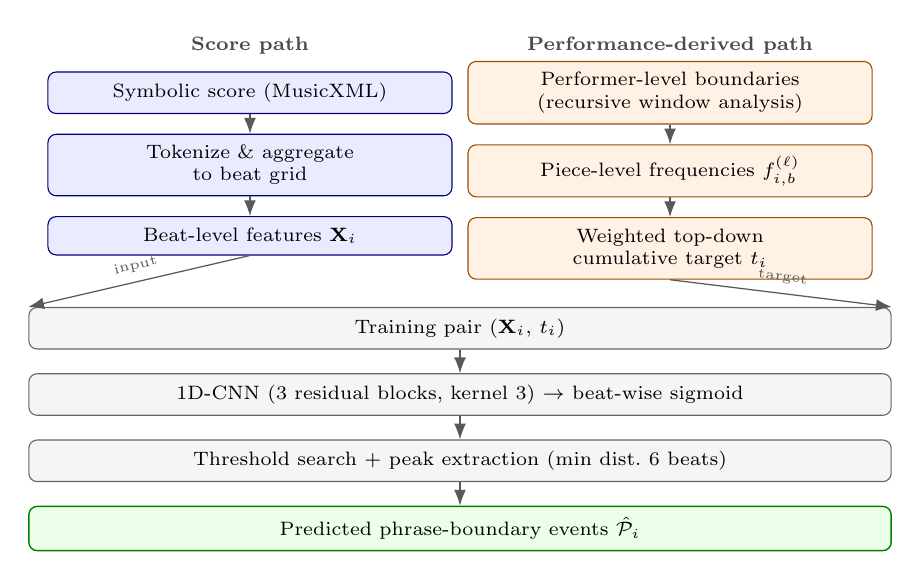
\begin{tikzpicture}[
    every node/.style={font=\scriptsize},
    score/.style={
      draw=blue!50!black, line width=0.4pt,
      fill=blue!8,
      rounded corners=3pt, align=center,
      text width=0.40\linewidth, inner sep=4pt
    },
    perf/.style={
      draw=orange!60!black, line width=0.4pt,
      fill=orange!10,
      rounded corners=3pt, align=center,
      text width=0.40\linewidth, inner sep=4pt
    },
    shared/.style={
      draw=black!60, line width=0.4pt,
      fill=gray!8,
      rounded corners=3pt, align=center,
      text width=0.88\linewidth, inner sep=4pt
    },
    output/.style={
      draw=green!50!black, line width=0.5pt,
      fill=green!8,
      rounded corners=3pt, align=center,
      text width=0.88\linewidth, inner sep=4pt
    },
    arrow/.style={-{Latex[length=2mm]}, line width=0.45pt, gray!70!black},
    grouplabel/.style={font=\scriptsize\bfseries, color=black!70}
  ]

    \node[grouplabel] (h1) at (-0.22\linewidth, 0.6) {Score path};
    \node[grouplabel] (h2) at ( 0.22\linewidth, 0.6) {Performance-derived path};

    \node[score] (score) at (-0.22\linewidth, 0) {Symbolic score (MusicXML)};
    \node[score, below=0.25cm of score] (tokenizer) {Tokenize \& aggregate\\to beat grid};
    \node[score, below=0.25cm of tokenizer] (features) {Beat-level features $\mathbf{X}_i$};

    \node[perf] (perf) at (0.22\linewidth, 0) {Performer-level boundaries\\(recursive window analysis)};
    \node[perf, below=0.25cm of perf] (freq) {Piece-level frequencies $f_{i,b}^{(\ell)}$};
    \node[perf, below=0.25cm of freq] (target) {Weighted top-down\\cumulative target $t_i$};

    \path (features.south) -- (target.south) coordinate[midway] (midpoint);
    \node[shared, below=0.50cm of midpoint] (pair)
      {Training pair $(\mathbf{X}_i,\, t_i)$};
    \node[shared, below=0.30cm of pair] (model)
      {1D-CNN (3 residual blocks, kernel 3) $\to$ beat-wise sigmoid};
    \node[shared, below=0.30cm of model] (decode)
      {Threshold search $+$ peak extraction (min dist.\ 6 beats)};
    \node[output, below=0.30cm of decode] (pred)
      {Predicted phrase-boundary events $\hat{\mathcal{P}}_i$};

    \draw[arrow] (score) -- (tokenizer);
    \draw[arrow] (tokenizer) -- (features);
    \draw[arrow] (perf) -- (freq);
    \draw[arrow] (freq) -- (target);
    \draw[arrow] (features.south) -- node[midway, sloped, above, font=\tiny] {input}
                 (pair.north west);
    \draw[arrow] (target.south)   -- node[midway, sloped, above, font=\tiny] {target}
                 (pair.north east);
    \draw[arrow] (pair) -- (model);
    \draw[arrow] (model) -- (decode);
    \draw[arrow] (decode) -- (pred);

  \end{tikzpicture}
  \caption{Method overview. The score path (blue) extracts beat-level features from MusicXML; the performance-derived path (orange) converts aligned tempo curves into a weighted top-down cumulative target. The two streams form $(\mathbf{X}_i, t_i)$ training pairs for a 1D-CNN, whose beat-wise sigmoid scores are decoded into discrete boundary events.}
  \label{fig:method_pipeline}
\end{figure}

\subsection{Score-Based Feature Representation}\label{subsec:score_features}

For each piece $i$, the model input is a beat sequence $\mathbf{X}_i = [\mathbf{x}_{i,1}, \ldots, \mathbf{x}_{i,B_i}]$ where $\mathbf{x}_{i,b}$ is a score-derived feature vector at beat $b$. The representation is entirely symbolic and therefore available at test time without any performance signal.

A lightweight MusicXML tokenizer first converts each score into note or chord-tone tokens with absolute onset, duration, pitch, part index, articulation flags, and tie status. Chords are expanded into per-pitch events, sorted by absolute onset, and aggregated to the beat grid. The resulting beat representation combines two parts. The note side summarizes what is locally sounding or articulated at the beat, including density, pitch, duration, onset spread, sustaining-note activity, and simple neighborhood contrasts. The MusicXML side summarizes notated structural context, including metrical position, barline proximity, time-signature and key cues, rests, ties, slurs, fermatas, dynamic markings, and tempo-text cues.

\subsection{Weighted Top-Down Cumulative Targets}\label{subsec:cumulative_targets}

Rather than training one model on all five raw layers at once, five cumulative detector targets are constructed, one per level. Each target $L_\ell$ contains all events from $L_5, L_4, \ldots, L_\ell$ combined, so each detector therefore recovers a consistent coarse-to-fine slice of the hierarchy rather than a single isolated layer.

Cumulative targets are assembled after performer averaging. Starting from $L_5$, layer-5 events are added, then layer-4 events, and so on down to layer-1, using the same merge rule throughout: if a newly added finer-level event falls within one beat of an already retained coarser event, it is absorbed into that location and the larger weighted value is kept there; otherwise it remains as a separate event. The component weights are $1.00, 0.64, 0.46, 0.28, 0.16$ for layers $5,4,3,2,1$, respectively.

\subsection{Boundary Prediction Model}\label{subsec:model}

Boundary prediction is modeled as sequence tagging on the piece-level beat grid. Given $\mathbf{X}_i$, the network outputs one logit per beat, interpreted after a sigmoid as the score for the currently selected detector target. Separate runs are trained for each of $L_1, \ldots, L_5$, sharing the same input representation and the same architecture.

The model is a 1D convolutional neural network with three residual blocks. Each block contains two 1D convolutions of kernel size 3 (dilation 1), batch normalization, GELU activation, dropout 0.2, and a residual skip connection. All three blocks use 64 channels, and a final $1\times 1$ convolution maps the last hidden representation to a single beat-level logit. Phrase boundaries depend on short- to medium-range local context and require beat-aligned outputs on variable-length sequences, which this architecture provides directly; an ablation with dilation factors $(1,2,4)$ did not improve over the non-dilated CNN (Section~\ref{subsec:outer_results}).

\subsection{Training Objective}\label{subsec:training_objective}

All feature dimensions are standardized using statistics estimated only from the training partition of the current fold. Sequences are padded within each mini-batch, with a binary mask $m_{i,b}$ excluding padding positions from the loss. With beat-level logits $z_{i,b}$ and weighted cumulative targets $t_{i,b}$, the model optimizes a masked weighted binary cross-entropy objective
\begin{align}
\mathcal{L} = -\frac{1}{M}\sum_{i,b} m_{i,b}\Big[ &w^{+} t_{i,b} \log \sigma(z_{i,b}) \notag\\
&+ (1{-}t_{i,b}) \log\big(1{-}\sigma(z_{i,b})\big) \Big],
\end{align}
where $\sigma$ is the sigmoid function, $M = \sum_{i,b} m_{i,b}$ is the total number of valid beats, and $w^{+}$ is a per-fold positive weight set to the negative-to-positive target mass ratio. Beats whose piece-level target frequency falls below $0.05$ are suppressed during training.

The decision threshold is selected by grid search over 37 evenly spaced values in $[0.05, 0.95]$ on the validation fold, maximizing weighted recall subject to a minimum union-precision floor of $0.85$ for $L_1, \ldots, L_4$ and $0.80$ for $L_5$ (relaxed because reference events at the coarsest level are sparse and the stricter floor empirically left too few valid operating points). At inference time, sigmoid scores are converted into discrete events by peak extraction with a minimum distance of six beats; matches against reference events use a one-beat tolerance.

\section{Experiments and Results}\label{sec:experiments}

\subsection{Experimental Protocol}\label{subsec:protocol}

The fixed outer test set consists of the three Mazurkas M06-1, M06-2, and M06-3; the remaining 41 pieces form the development pool. For each detector target and each of five random seeds, leave-one-piece-out inner validation is performed on the development pieces, after which a clean outer fit is performed on all 41 of them. The outer test does not re-tune on the held-out Mazurkas: the decision threshold and the number of training epochs are frozen to the mean of the fold-wise selected values from inner validation, so the three M06 pieces remain untouched until the final evaluation.

Three complementary event-level metrics are reported. Let $\mathcal{P}_i$ be the predicted event set for piece $i$, $\mathcal{U}_i$ the set of reference beats with nonzero frequency target, and $\mathcal{M}_i$ a greedy set of matched prediction-reference pairs within the one-beat tolerance. \emph{Union precision} (U.P.) is the fraction of $\mathcal{P}_i$ matched against $\mathcal{U}_i$. \emph{Consensus recall} (C.R.) counts only reference events with frequency target $\geq 0.5$. \emph{Weighted recall} measures the piece-level frequency mass recovered by matched predictions,
\begin{equation}
\mathrm{WR} =
\frac{\sum_i \sum_{(p,u)\in\mathcal{M}_i} f_{i,u}}
     {\sum_i \sum_{u\in\mathcal{U}_i} f_{i,u}}.
\end{equation}
\emph{Pred. Events} in Table~\ref{tab:outer_merge56_results} denotes the mean cardinality of $\mathcal{P}_i$ across outer pieces and seeds.

\subsection{Quantitative Results on the Outer Mazurkas}\label{subsec:outer_results}

Table~\ref{tab:outer_merge56_results} summarizes clean outer results, averaged over five random seeds and pooled across the three outer Mazurkas. Across the five detector targets, mean union precision is $0.872$, weighted recall is $0.405$, and consensus recall is $0.512$, so the model returns usable boundary events at every level without collapsing into either empty outputs or near-uniform overprediction. Event density also changes in the expected direction: the mean number of predicted events drops from roughly $125$ at $L_1$ to $27$ at $L_5$, matching the intended coarse-to-fine ordering.

Table~\ref{tab:outer_baselines_multiseed} reports the corresponding clean-outer comparison on the same M06 split. The weighted top-down target construction improves logistic regression over simple union ($0.776/0.257$ vs.\ $0.757/0.215$ in mean U.P./W.R.), supporting the cumulative target design independently of the sequence model. Replacing the 1D-CNN with a dilated TCN with dilation factors $(1,2,4)$ yields essentially the same union precision and a slightly higher weighted recall ($0.417$ vs.\ $0.405$) but a meaningfully lower consensus recall ($0.472$ vs.\ $0.512$); the simpler architecture is adopted as the main model. Feature ablations show that note-only features dominate at fine levels, whereas xml-only features become more useful at the coarsest level, where $L_5$ weighted recall is $0.367$ for xml-only versus $0.073$ for note-only.

All baselines and ablations share the same outer protocol, target labels, threshold-search procedure, and event extraction settings. The LBDM rule-based baseline computes beat salience from local pitch, IOI, and rest cues on the top and bottom score voices, summed across voices and decoded with the same threshold-search and peak-extraction procedure as the trained models.

\begin{table}[t]
  \centering
  \resizebox{\columnwidth}{!}{%
  \begin{tabular}{lcccc}
    \hline
    Target & Union Prec. & Weighted Rec. & Consensus Rec. & Pred. Events \\
    \hline
    $L_1$ & 0.913 & 0.510 & 0.560 & 125.0 \\
    $L_2$ & 0.864 & 0.515 & 0.480 & 124.0 \\
    $L_3$ & 0.872 & 0.340 & 0.320 & 63.5 \\
    $L_4$ & 0.870 & 0.269 & 0.480 & 32.0 \\
    $L_5$ & 0.842 & 0.391 & 0.720 & 27.0 \\
    \hline
  \end{tabular}%
  }
  \caption{Clean outer results for the weighted top-down cumulative hierarchy. Values are means over five random seeds, pooled across outer pieces M06-1, M06-2, and M06-3. }
  \label{tab:outer_merge56_results}
\end{table}

\begin{table}[t]
  \centering
  \resizebox{\columnwidth}{!}{%
  \begin{tabular}{l|ccc|ccc|ccc}
    \hline
    Setting & \multicolumn{3}{c|}{Mean across $L_1$--$L_5$} & \multicolumn{3}{c|}{$L_4$} & \multicolumn{3}{c}{$L_5$} \\
    \cline{2-10}
     & U.P. & W.R. & C.R. & U.P. & W.R. & C.R. & U.P. & W.R. & C.R. \\
    \hline
    \textbf{1D-CNN, all features} & \textbf{0.872} & 0.405 & \textbf{0.512} & 0.870 & 0.269 & \textbf{0.480} & \textbf{0.842} & \textbf{0.391} & \textbf{0.720} \\
    Dilated TCN ablation & 0.869 & \textbf{0.417} & 0.472 & \textbf{0.880} & \textbf{0.282} & 0.440 & 0.836 & 0.367 & 0.640 \\
    \hline
    LogReg, all features & 0.776 & 0.257 & 0.120 & 0.750 & 0.130 & 0.000 & 0.613 & 0.115 & 0.000 \\
    LogReg, simple-union targets & 0.757 & 0.215 & 0.339 & 0.643 & 0.108 & 0.000 & 0.613 & 0.115 & 0.000 \\
    LogReg, note-only features & 0.733 & 0.245 & 0.120 & 0.609 & 0.060 & 0.000 & 0.480 & 0.073 & 0.000 \\
    LogReg, xml-only features & 0.684 & 0.283 & 0.400 & 0.667 & 0.194 & 0.200 & 0.571 & 0.367 & 0.600 \\
    LBDM, all features & 0.615 & 0.250 & 0.080 & 0.543 & 0.172 & 0.000 & 0.435 & 0.139 & 0.000 \\
    \hline
  \end{tabular}%
  }
  \caption{Clean-outer baseline and ablation summary on M06-1, M06-2, and M06-3, means over five random seeds. U.P., W.R., and C.R. denote union precision, weighted recall, and consensus recall. All settings use the weighted top-down cumulative target unless otherwise stated (the \emph{simple-union targets} row replaces the target construction).}
  \label{tab:outer_baselines_multiseed}
\end{table}

\subsection{Controlled Human Evaluation}\label{subsec:human_eval}

To assess whether the predicted hierarchy aligns with musical intuition, a controlled blind evaluation was conducted on the three clean-outer Mazurkas and on the first movement of Mozart's Piano Sonata in G major, K.~283. For each piece, all model-predicted boundaries were rendered onto the score using identical visual markings, and 10 randomly placed positions were added as negative controls. Three musicians of varying training participated: Le, an eight-year piano teacher at the School of Music Education of the Wuhan Conservatory of Music; Jin, a graduate piano major at the Central Conservatory of Music with fifteen years of piano experience; and Li, an amateur with more than ten years of piano playing. All three rated the Mazurkas; for the Mozart movement, ratings were collected only from Jin and Li. All raters were blind to which markings were model-predicted and which were random controls. The study received ethics approval from the institutional review board prior to data collection, and all participants gave informed consent.

Each marking was labeled on a three-point scale through expressive slowdown: \emph{should} (required), \emph{may} (acceptable but not required), or \emph{should-not} (would disrupt performance). Raters could also add unmarked boundaries they considered required. \emph{Strict} precision counts only \emph{should}; \emph{lenient} precision counts \emph{should} or \emph{may}.

Table~\ref{tab:human_precision} summarizes acceptance rates pooled across the three Mazurkas. All three raters assign \emph{should} to zero of the 28 random controls, providing a clean negative control. Lenient acceptance of model boundaries reaches \(0.925\) (Le), \(0.866\) (Jin), and \(0.925\) (Li), substantially above the lenient acceptance of random controls; Fisher exact tests reject the null at \(p<10^{-4}\) for all three raters. Strict precision varies more across raters (\(0.216\), \(0.149\), \(0.075\)), reflecting differences in musical training and willingness to commit to a strong \emph{should} label, but every rater's strict precision on random controls is exactly zero.

Table~\ref{tab:human_layer} examines a stricter precision variant requiring at least two of the three raters to agree. The \(\geq 2\)-\emph{should} rate increases monotonically with predicted hierarchy depth, from $0\%$ at $L_1$/$L_2$ to $27.3\%$ at $L_5$, and remains at zero on random controls. The all-three-lenient rate reaches $97.0\%$ at $L_5$, meaning that almost every position the model predicts at the coarsest level is accepted by all three raters as at least musically permissible. This monotonic alignment supports the claim that the predicted layer indices carry structural meaning rather than acting as arbitrary depth labels.

Across the three Mazurkas, the raters added 50 positions in total (15 by Le, 28 by Jin, 7 by Li). Le marked 7 added positions as \emph{should}; Jin marked none; Li marked one. Combining the model's recovered \emph{should} boundaries with each rater's added \emph{should} positions yields a strict recall of \(0.81\) (Le), \(1.00\) (Jin), and \(0.91\) (Li); lenient recall is \(0.89\), \(0.81\), and \(0.95\).

Three-class Fleiss' \(\kappa\) across the three raters is \(0.46\) on the 162 numbered positions, rising to \(0.54\) for the binary \emph{should}-versus-rest contrast. The three raters differ in baseline stringency---Jin rejects \(75\%\) of random controls, Li \(64\%\), and Le \(43\%\)---but all produce zero strict false positives on random and accept the great majority of model boundaries leniently. This level of agreement is consistent with prior reports of moderate inter-annotator agreement on phrase-boundary tasks~\cite{McFee2017HierarchicalAnnotations,Wang2017CrowdsourcingSegmentation} and is itself part of the motivation for using performance-derived supervision.

The trained detectors were also applied qualitatively to Mozart K.~283 (100 model-predicted boundaries, 10 random controls), with ratings from Jin and Li only. The hierarchy ordering is preserved on this stylistically different work: the both-rater lenient rate increases monotonically from $6.5\%$ at $L_2$ to $92.3\%$ at $L_5$, and the both-rater \emph{should} rate at $L_5$ reaches $23.1\%$. Absolute lenient precision is lower than on Mazurka and rater-dependent ($0.51$ for Jin, $0.82$ for Li); the Mozart result is treated as a hierarchy-ordering check rather than as a precision claim, and broader cross-corpus evaluation is left to future work.

\begin{table}[t]
  \centering
  \resizebox{\columnwidth}{!}{%
  \begin{tabular}{lccc|ccc}
    \hline
     & \multicolumn{3}{c}{Strict P} & \multicolumn{3}{c}{Lenient P} \\
    \cline{2-7}
    Source & Le & Jin & Li & Le & Jin & Li \\
    \hline
    Model boundary ($n=134$) & 0.216 & 0.149 & 0.075 & 0.925 & 0.866 & 0.925 \\
    Random control ($n=28$)  & 0.000 & 0.000 & 0.000 & 0.571 & 0.250 & 0.357 \\
    \hline
    Lift over random         & +0.216 & +0.149 & +0.075 & +0.354 & +0.616 & +0.568 \\
    \hline
  \end{tabular}%
  }
  \caption{Precision of model-predicted boundaries vs randomly placed controls under the controlled human evaluation, pooled across M06-1, M06-2, and M06-3. All three raters assign zero \emph{should} labels to random controls and accept the large majority of model boundaries leniently.}
  \label{tab:human_precision}
\end{table}

\begin{table}[t]
  \centering
  \resizebox{\columnwidth}{!}{%
  \begin{tabular}{lccccc}
    \hline
    Layer & $n$ & all-3 \emph{should} & $\geq 2$ \emph{should} & all-3 lenient & $\geq 2$ lenient \\
    \hline
    $L_1$ & 12 & 0.0\% & 0.0\% & 33.3\% & 75.0\% \\
    $L_2$ & 31 & 0.0\% & 0.0\% & 71.0\% & 93.5\% \\
    $L_3$ & 47 & 4.3\% & 8.5\% & 85.1\% & 97.9\% \\
    $L_4$ & 11 & 18.2\% & 18.2\% & 72.7\% & 90.9\% \\
    $L_5$ & 33 & \textbf{18.2\%} & \textbf{27.3\%} & \textbf{97.0\%} & \textbf{100.0\%} \\
    \hline
    Random  & 28 & 0.0\% & 0.0\% & 14.3\% & 39.3\% \\
    \hline
  \end{tabular}%
  }
  \caption{Multi-rater consensus acceptance, computed as the fraction of model boundaries on which the indicated number of raters agree, broken down by predicted level. Each position is reported at the coarsest cumulative target level $L_\ell$ at which the model predicts it; positions predicted at $L_5$ also appear in all finer levels by construction and are tabulated only once at $L_5$.}
  \label{tab:human_layer}
\end{table}


\subsection{Tempo-Curve Reconstruction}\label{subsec:reconstruction}

As preparation for a later audio-generation stage, this experiment tested whether the predicted hierarchical breakpoints could support a coarse reconstruction of formal tempo shape. Each performer tempo curve was converted to a per-performer z-score representation. Using only the 41 training Mazurkas, linear reconstruction coefficients were fit and applied on each outer piece. Three reconstructions were then compared: (i) thresholded performance-derived cumulative targets (upper bound), (ii) predicted events from all five detector levels ($L_1$--$L_5$) using coefficients fit on all five levels, and (iii) predicted events from high levels only ($L_4/L_5$) using coefficients refit with only $L_4/L_5$, with detector scores used as boundary strengths.

\begin{figure}[t]
  \centering
  
\includegraphics[width=\columnwidth]{M06-2_predicted_tempo_reconstruction_0_100_clean_with_l45_overlay.pdf}
  \caption{Local reconstruction example for M06-2 (beats 0--100). Gray envelopes summarize performer tempo distributions (outer min/max with denser central bands). Black: mean performer tempo. Red: reconstruction from all predicted levels ($L_1$--$L_5$). Orange dashed: reconstruction from $L_4/L_5$ only.}
  \label{fig:m06_2_reconstruction}
\end{figure}

Averaged over the three outer Mazurkas, the upper-bound reconstruction from performance-derived cumulative targets reaches correlation $0.682$ with the mean performer curves. All-level reconstruction from predicted events reaches mean correlation $0.518$ (RMSE $0.664$), while $L_4/L_5$-only reaches $0.483$ (RMSE $0.677$): high levels capture major phrase-scale motion (Figure~\ref{fig:m06_2_reconstruction}), and finer levels still improve overall fit. The reconstructions do not match performer means beat by beat but recover large-scale rises and falls, supporting downstream use as a control signal for audio generation.

\section{Conclusion}\label{sec:conclusion}

This paper presented a score-only model for hierarchical phrase-boundary prediction trained from performance-derived supervision. Aligned Mazurka tempo curves are reorganized into a weighted top-down cumulative target that encodes hierarchical consistency in label space, allowing a single 1D-CNN to produce five coarse-to-fine detectors nested by design. Under a strict outer-piece protocol on M06-1, M06-2, and M06-3, the model achieves mean union precision $0.872$, weighted recall $0.405$, and consensus recall $0.512$, and ablations show that the weighted top-down target outperforms a simple-union construction independently of the sequence model.

A controlled blind evaluation by three musicians of varying training shows that random control markers receive zero \emph{should} labels from any rater while $87\%$--$93\%$ of model-predicted boundaries are accepted as at least musically permissible, with strong-consensus acceptance increasing monotonically with predicted depth; the layer ordering is also preserved on Mozart K.~283. A post hoc tempo-curve reconstruction analysis additionally indicates that the predicted hierarchy retains enough structural information to recover the broad shape of mean expressive tempo curves. Together, these results support performance-derived supervision as a viable substitute for hard-to-collect phrase annotations, and the predicted hierarchy as an interpretable structural module for expressive-performance generation and as a readable aid for piano learning and performance preparation.

Future work will pursue three directions: generating audio from the reconstructed tempo curves and evaluating it in perceptual listening experiments; expanding the training pool to more meters, styles, and composers, which may also help close the systematic gap on weak-beat phrase endings observed in the human evaluation; and rendering more suitable visual markings on the score itself.

\bibliography{ISMIRchangheng}

\end{document}
